\section{Introduzione}
La specifica della Prova Finale (Progetto di Reti Logiche) 2019 è ispirata al metodo di codifica a bassa dissipazione di potenza denominato \textit{Working Zone}.\newline
Tale metodo è pensato per il Bus Indirizzi e si usa per trasformare il valore di un indirizzo, quando questo viene trasmesso, se appartiene a certi intervalli (detti appunto working-zone). Una working-zone è definita come un intervallo di indirizzi di dimensione fissa ($D_{wz}$) che parte da un indirizzo base. All'interno dello schema di codifica possono esistere multiple working-zone ($N_{wz}$).

\subsection{Obiettivo del progetto}
Dati gli indirizzi base delle working-zone e l'indirizzo da codificare, si vuole implementare un componente hardware descritto in VHDL in grado di leggere l'indirizzo da codificare e gli indirizzi base delle working-zone, verificare l'appartenenza dell'indirizzo da codificare a tali working-zone e produrre l'indirizzo opportunamente codificato in uscita.
In pratica, il modulo da sviluppare si comporta come un \textbf{encoder} di indirizzi.

\subsection{Specifica generale}
Si consideri l'indirizzo da trasmettere $ADDR$. Lo schema di codifica implementato è il seguente:
\begin{itemize}
	\item se $ADDR$ non appartiene a nessuna Working Zone \textbf{[WZ MISS]}, verrà trasmesso un bit addizionale ${WZ}_{BIT}=0$ concatenato ad $ADDR$ (${WZ}_{BIT}$ \& $ADDR$, dove \& è il simbolo di concatenazione);
	
		\begin{figure}[!htb]
			\tikzstyle{int}=[draw, fill=black!10, minimum size=4em]
\tikzstyle{init} = [pin edge={to-,thin,black}]

\centering

\begin{tikzpicture}[node distance=6cm,auto,>=latex']
\node [int] (a) {ENCODER};
\node (b) [left of=a,node distance=5cm]{SOURCE};
\node (end) [right of=a, node distance=8cm]{DEST};
\path[->] (b) edge node {$ADDR$} (a);
\draw[->] (a) edge node {$0$ \& $ADDR$} (end);
\end{tikzpicture}
			\caption{codifica di un indirizzo non appartenente a nessuna WZ.}
			\label{fig:addr_no_wz}
		\end{figure}

	\item se $ADDR$ appartiene ad una Working Zone \textbf{[WZ HIT]}, verrà trasmesso ${WZ}_{BIT}=1$ concatenato a due valori ${WZ}_{NUM}$ e ${WZ}_{OFFSET}$, rappresentanti rispettivamente:
	\begin{itemize}
		\item il numero della working-zone al quale l'indirizzo appartiene, codificato in binario;
		
		\item l'offset rispetto all'indirizzo di base della working-zone, codificato come one-hot.
	\end{itemize}

	
	
	\begin{figure}[!htb]
		\input{figures/encoding_address_2}	
		\caption{codifica di un indirizzo appartenente ad una WZ.}
		\label{fig:addr_in_wz}
	\end{figure}
\end{itemize}

Si considerino 7 bit per l'indirizzo da codificare (quindi indirizzi validi da 0 a 127).\newline
Il numero di working-zone è 8 ($N_{wz}=8$) mentre la dimensione della working-zone è di 4 indirizzi incluso quello base ($D_{wz}=4$). Questo comporta che l'indirizzo codificato sarà composto da 8 bit: 1 bit per ${WZ}_{BIT}$ + 7 bit per $ADDR$, oppure 1 bit per ${WZ}_{BIT}$, 3 bit per codificare in binario a quale tra le 8 working-zone l'indirizzo appartiene, e 4 bit per codificare one-hot il valore dell'offset di $ADDR$ rispetto all'indirizzo base.\newline

\textbf{Esempio}: codifica di $ADDR$=33, sapendo che la WZ 3 ha come indirizzo di base 31.
\begin{figure}[!htb]
	\centering
	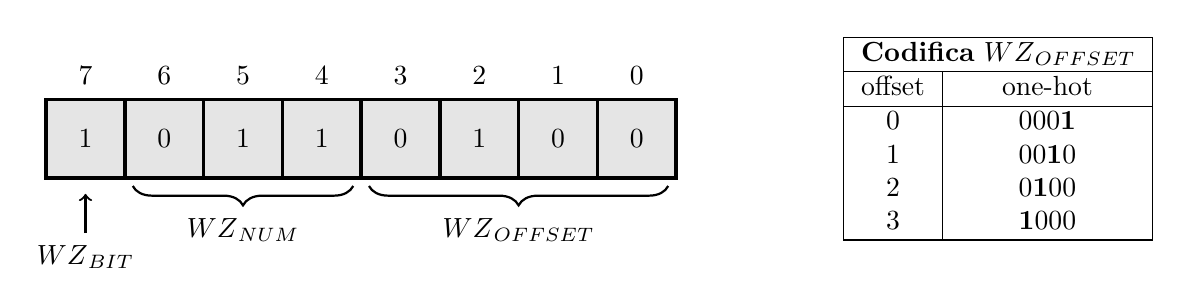
\begin{tikzpicture}[box/.style={fill=black!10, rectangle,draw=black, very thick, minimum size=1cm}]
	
	\foreach \i in {0,...,7} {
		\node at (8-\i-1,0.8){\i};
	}
	
	\foreach \y [count=\x] in {1,0,1,1,0,1,0,0} {
		\node[box] at (\x-1,0){\y};
	}

	\draw[decorate,decoration={brace, amplitude=7pt, raise=0pt, mirror}, thick] (0.6,-.6) -- node[below=8pt]{${WZ}_{NUM}$} (3.4,-.6);
	\draw[decorate,decoration={brace, amplitude=7pt, raise=0pt, mirror}, thick] (3.6,-.6) -- node[below=8pt]{${WZ}_{OFFSET}$} (7.4,-.6);
	\draw[->, thick] (0,-1.2) --  node[below=2pt,yshift=-2mm]{${WZ}_{BIT}$} (0,-.7);

	\node[text width=4cm, anchor=west, right] at (9.5,0) {	
		\begin{tabular}{ |c|c| }
		\hline
		\multicolumn{2}{|c|}{\textbf{Codifica ${WZ}_{OFFSET}$}} \\
		\hline
		offset & one-hot\\
		\hline
		0 & 000\textbf{1}\\
		1 & 00\textbf{1}0\\
		2 & 0\textbf{1}00\\
		3 & \textbf{1}000\\
		\hline
		\end{tabular}
	};
\end{tikzpicture}

	\caption{ADDR appartiene alla WZ 3, con offset 2 (in one-hot).}
	\label{fig:es_addr_in_wz}
\end{figure}



\subsection{Interfaccia del componente}
Il componente descritto possiede la seguente interfaccia:

\begin{lstlisting}[basicstyle=\small, language=VHDL]
entity project_reti_logiche is
port (
	i_clk 		: in std_logic;
	i_start 	: in std_logic;
	i_rst 		: in std_logic;
	i_data 		: in std_logic_vector(7 downto 0);
	o_address 	: out std_logic_vector(15 downto 0);
	o_done 		: out std_logic;
	o_en 		: out std_logic;
	o_we 		: out std_logic;
	o_data 		: out std_logic_vector(7 downto 0)
);
end project_reti_logiche;
\end{lstlisting}


In particolare:
\begin{itemize}
	\item \lstinline[columns=fixed]{i_clk} è il segnale di \lstinline[columns=fixed]{CLOCK} in ingresso generato dal Test Bench;
	
	\item \lstinline[columns=fixed]{i_start} è il segnale di \lstinline[columns=fixed]{START} generato dal Test Bench;
	
	\item \lstinline[columns=fixed]{i_rst} è il segnale di \lstinline[columns=fixed]{RESET} che inizializza la macchina pronta per ricevere il primo segnale di \lstinline[columns=fixed]{START};
	
	\item \lstinline[columns=fixed]{i_data} è il segnale (vettore) che arriva dalla memoria in seguito ad una richiesta di lettura;
	
	\item \lstinline[columns=fixed]{o_address} è il segnale (vettore) di uscita che manda l'indirizzo alla memoria;
	
	\item \lstinline[columns=fixed]{o_done} è il segnale di uscita che comunica la fine dell'elaborazione e il dato di uscita scritto in memoria;
	
	\item \lstinline[columns=fixed]{o_en} è il segnale di \lstinline[columns=fixed]{ENABLE} da dover mandare alla memoria per poter comunicare (sia in lettura che in scrittura);
	
	\item \lstinline[columns=fixed]{o_we} è il segnale di \lstinline[columns=fixed]{WRITE ENABLE} da dover mandare alla memoria (=1) per poter scriverci. Per leggere da memoria esso deve essere 0;
	
	\item \lstinline[columns=fixed]{o_data} è il segnale (vettore) di uscita dal componente verso la memoria.
\end{itemize}

\subsection{Dati e memoria}
Il componente dovrà gestire la comunicazione con una memoria ausiliaria sulla quale saranno presenti i dati in ingresso e andranno salvati quelli in uscita.\newline
I dati, ciascuno di dimensione 8 bit, sono memorizzati sulla memoria con indirizzamento al Byte partendo dalla posizione 0.
Anche l'indirizzo da codificare che è da specifica di 7 bit viene memorizzato su 8 bit (il valore dell'ottavo bit sarà sempre zero).

La memoria è così organizzata:
\begin{itemize}
	\item Le posizioni da 0 a 7 sono usate per memorizzare gli otto indirizzi base delle working-zone;
	
	\item La posizione 8 è usata per memorizzare il valore (indirizzo) da codificare ($ADDR$);
	
	\item La posizione 9 è usata per scrivere il valore codificato in uscita.
\end{itemize}

\begin{figure}[!htb]
	\centering
	\tikzstyle{freecell}=[fill=black!10]
\tikzstyle{occupiedcell}=[fill=black!10]

\renewcommand{\llcell}[3]{
	\addtocounter{cellnb}{-#1}
	\setcounter{ptrnb}{0}
	\draw[#2] (0,\value{cellnb}) +(-2.8,-.5) rectangle +(2.8,-.5+#1);
	\draw (0,\value{cellnb}+#1/2-0.5)  node(currentcell) {#3};
}

\renewcommand{\finishframe}[1]{
	\draw[snake=brace, line width=0.6pt, segment amplitude=8pt]
	(-2.8,\value{cellnb}-0.5) -- (-2.8,\value{startframe}-0.5);
	\draw (-5.4cm,\value{cellnb}*0.5+\value{startframe}*0.5-0.7) node
	{\parbox{3cm}{%
	\begin{flushright}
		#1
	\end{flushright}}};
}

\renewcommand{\separator}[1][freecell,very thick]{
	\draw[#1] (0,\value{cellnb}) +(-2.8,-.5) -- +(2.8,-.5);
}

\renewcommand{\cellcom}[1]{
	\draw (3.1,\value{ptrnb}*0.5+\value{cellnb}) node[anchor=west] {#1};
	\addtocounter{ptrnb}{1}
}

\renewcommand{\stackbottom}[1][freecell]{
	\addtocounter{cellnb}{-1}
	\draw[#1] (0,\value{cellnb})
	+(-2.8,-.5) -- +(-2.8,+.5) -- +(2.8,+.5) -- +(2.8,-.5);
	\draw (0,\value{cellnb}) node{...};
}


\begin{tikzpicture}[scale=0.8]
	\small
	\cell[draw=none]{RAM} \cellcom{Indirizzo}
	\startframe
	\cell{Indirizzo Base WZ 0}        \cellcom{0}
	\cell{Indirizzo Base WZ 1}        \cellcom{1}
	\cell{...} \cellcom{...}
	\cell{Indirizzo Base WZ 7} \cellcom{7}
	\cell{Indirizzo da codificare}     \cellcom{8}
	\finishframe{Input del componente}
	\separator
	\cell{Indirizzo codificato} \cellcom{9}
	\stackbottom{}
	
	\draw[->, thick] (-3.8,-7) --  node[left=2pt,xshift=-4mm]{Output del componente} (-2.8,-7);
	
\end{tikzpicture}

	\caption{indirizzi della RAM rilevanti.}
	\label{fig:ram_1}
\end{figure}

%\input{figures/test}

